% Digital Logic Report Template
% Created: 2020-01-10, John Miller

%==========================================================
%=========== Document Setup  ==============================

% Formatting defined by class file
\documentclass[11pt]{article}

% ---- Document formatting ----
\usepackage[margin=1in]{geometry}	% Narrower margins
\usepackage{booktabs}				% Nice formatting of tables
\usepackage{graphicx}				% Ability to include graphics

%\setlength\parindent{0pt}	% Do not indent first line of paragraphs 
\usepackage[parfill]{parskip}		% Line space b/w paragraphs
%	parfill option prevents last line of pgrph from being fully justified

% Parskip package adds too much space around titles, fix with this
\RequirePackage{titlesec}
\titlespacing\section{0pt}{8pt plus 4pt minus 2pt}{3pt plus 2pt minus 2pt}
\titlespacing\subsection{0pt}{4pt plus 4pt minus 2pt}{-2pt plus 2pt minus 2pt}
\titlespacing\subsubsection{0pt}{2pt plus 4pt minus 2pt}{-6pt plus 2pt minus 2pt}

% ---- Hyperlinks ----
\usepackage[colorlinks=true,urlcolor=blue]{hyperref}	% For URL's. Automatically links internal references.

% ---- Code listings ----
\usepackage{listings} 					% Nice code layout and inclusion
\usepackage[usenames,dvipsnames]{xcolor}	% Colors (needs to be defined before using colors)

% Define custom colors for listings
\definecolor{listinggray}{gray}{0.98}		% Listings background color
\definecolor{rulegray}{gray}{0.7}			% Listings rule/frame color

% Style for Verilog
\lstdefinestyle{Verilog}{
	language=Verilog,					% Verilog
	backgroundcolor=\color{listinggray},	% light gray background
	rulecolor=\color{blue}, 			% blue frame lines
	frame=tb,							% lines above & below
	linewidth=\columnwidth, 			% set line width
	basicstyle=\small\ttfamily,	% basic font style that is used for the code	
	breaklines=true, 					% allow breaking across columns/pages
	tabsize=3,							% set tab size
	commentstyle=\color{gray},	% comments in italic 
	stringstyle=\upshape,				% strings are printed in normal font
	showspaces=false,					% don't underscore spaces
}

% How to use: \Verilog[listing_options]{file}
\newcommand{\Verilog}[2][]{%
	\lstinputlisting[style=Verilog,#1]{#2}
}




%======================================================
%=========== Body  ====================================
\begin{document}

\title{ELC 2137 Lab 08: 4-digit Display}
\author{Yiting Wang}

\maketitle


\section*{Summary}

Type the summary of your experiment and results here.  


\section*{Q\&A}

There is no question in the lab 08 assignment.


\section*{Results}

	Firgure 1 is the simulation waveform and ERT of the mux2.\\

\begin{figure}[ht]\centering
	\begin{tabular}{l|rrrr|rrrr|rrrr}
		Time (ns): & 0 & 10 & 20 & 30 & 40 & 50 & 60 & 110 & 120 & 130 & 140 & 150 \\
		\midrule
		num & 0000 & 0001 & 0010 & 0011 & 0100 & 0101 & 0110 & 1011 & 1100 & 1101 & 1110 & 1111 \\
		\midrule
		out & 0000 & 0001 & 0010 & 0011 & 0100 & 1000 & 1001 & 1110 & 1111 & 0000 & 0001 & 0010 \\
		\bottomrule
	\end{tabular}\medskip
	
	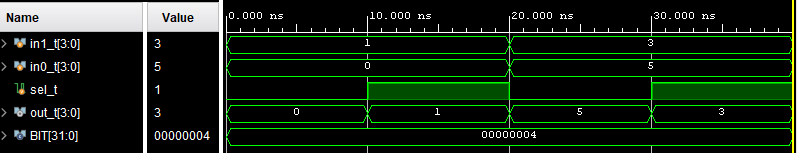
\includegraphics[width=1\textwidth]{mux2_simulation}
	\caption{the simulation waveform and ERT of the mux2}
	\label{fig:mux2_simulation}
\end{figure}


Firgure 2 is the simulation waveform and ERT of the mux4.\\
.\\
\begin{figure}[ht]\centering
	\begin{tabular}{l|rrr|rrrr}
		Time (ns): & 0 & 10 & 20 & 600 & 610 & 620 & 630 \\
		\midrule
		Bin & 000000 & 000001 & 000010 & 111100 & 111101 & 111110 & 111111 \\
		\midrule
		ones & 0000 & 0001 & 0010 & 0000 & 0001 & 0010 & 0011 \\
		tens & 0000 & 0000 & 0000 & 0110 & 0110 & 0110 & 0110 \\
		\bottomrule
	\end{tabular}\medskip
	
	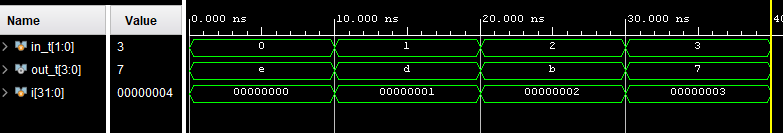
\includegraphics[width=1\textwidth]{anode_decoder_simulation}
	\caption{the simulation waveform and ERT of the mux4}
	\label{fig:mux4_simulation}
\end{figure}


Firgure 3 is the simulation waveform and ERT of the anode decoder.\\
.\\
\begin{figure}[ht]\centering
	\begin{tabular}{l|rrrr|rrrr|rr}
		Time (ns): & 0 & 10 & 20 & 30 & 40 & 50 & 20430 & 20440 & 20450 & 20460 \\
		\midrule
		Bin & 000 & 001 & 002 & 003 & 004 & 005 & 7fb & 7fc & 7fd & 7fe \\
		\midrule
		ones & 0000 & 0001 & 0010 & 0011 & 0100 & 0101 & 0011 & 0100 & 0101 & 0110 \\
		tens & 0000 & 0000 & 0000 & 0000 & 0000 & 0000 & 0100 & 0100 & 0100 & 0100 \\
		hund & 0000 & 0000 & 0000 & 0000 & 0000 & 0000 & 0000 & 0000 & 0000 & 0000 \\
		thou & 0000 & 0000 & 0000 & 0000 & 0000 & 0000 & 0010 & 0010 & 0010 & 0010 \\
		\bottomrule
	\end{tabular}\medskip
	
	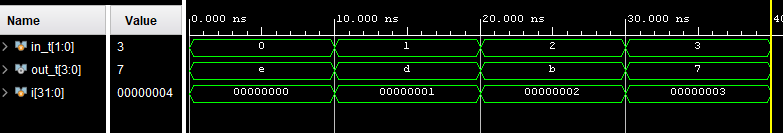
\includegraphics[width=1\textwidth]{anode_decoder_simulation}
	\caption{the simulation waveform and ERT of the anode decoder}
	\label{fig:anode_decoder_simulation}
\end{figure}

This is the picture of my board which showing a value on the first digit\\
\begin{center}
	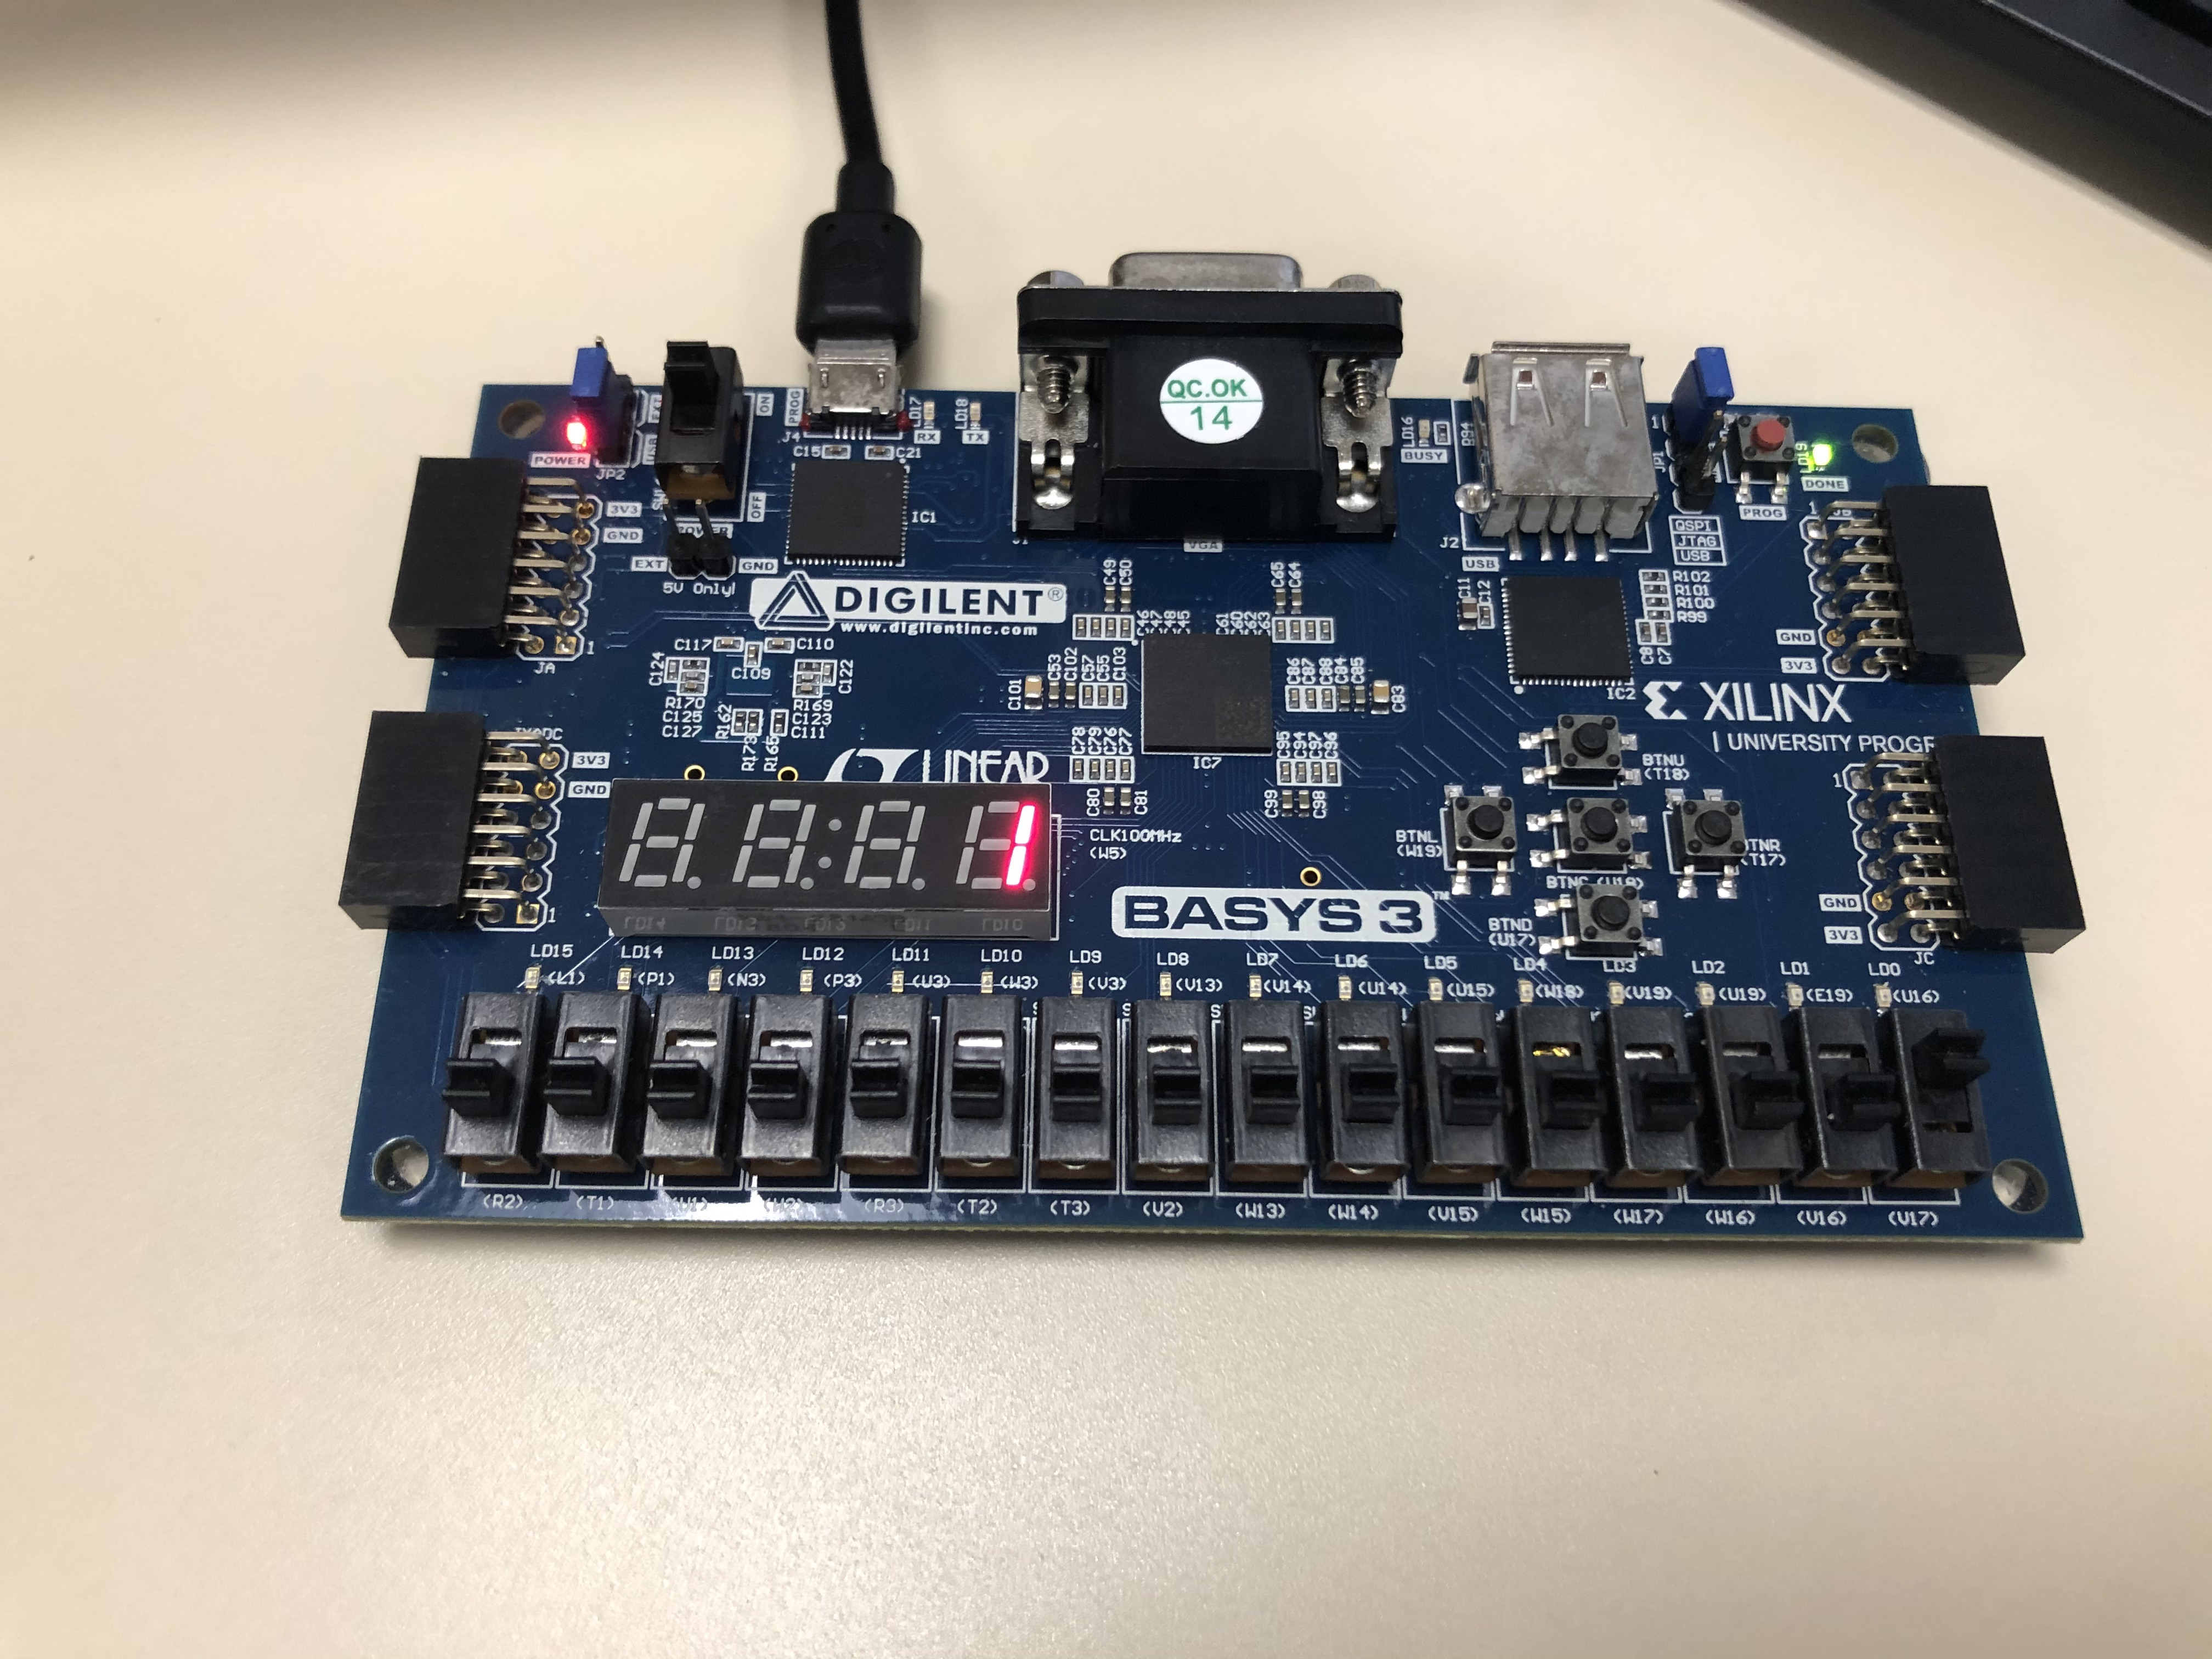
\includegraphics[width=0.7\textwidth]{board1}
\end{center}


\section*{Code}

\subsection*{File Inclusion}
\Verilog[caption=mux2 Verilog code,label=code:file_ex]{mux2.sv}

\subsection*{File Inclusion}
\Verilog[caption=mux2 Test Benches Verilog code,label=code:file_ex]{mux2_test.sv}


\subsection*{File Inclusion}
\Verilog[caption=mux4 Verilog code,label=code:file_ex]{mux4.sv}

\subsection*{File Inclusion}
\Verilog[caption=mux4 Test Benches Verilog code,label=code:file_ex]{mux4_test.sv}


\subsection*{File Inclusion}
\Verilog[caption=anode decoder Verilog code,label=code:file_ex]{anode_decoder.sv}

\subsection*{File Inclusion}
\Verilog[caption=anode decoder Test Benches Verilog code,label=code:file_ex]{anode_decoder_test.sv}


\subsection*{File Inclusion}
\Verilog[caption=sseg4 Verilog code,label=code:file_ex]{sseg4.sv}

\subsection*{File Inclusion}
\Verilog[caption=sseg4 manual Verilog code,label=code:file_ex]{sseg4_manual.sv}



\end{document}
